% !TEX root = ../../../thesis.tex
We suspect that the sharp edges in the CPR from sample CP2 might be caused by multi-valued measurements. $\beta_{rf}\approx 0.91$ for the previous sample according to our result. In order to get a $\beta_{\text{rf}} < 0.9$ we decided to lower the inductance. Alternatively we could have lowered the critical current. To do so we could have created the junction's loop with a smaller inner diameter. 

Additionally, in order to more accurately control the flux through the dc-SQUID we add a modulation line. This allows us to bias the dc-SQUID in the linear regime without the need for an external field. Furthermore it also enables the use for a flux-locked loop (FLL). The implementation of the modulation line is based on~\cite{linYBaCuNano2020}.

As an alternative we considered making a third loop identical to the junction's loop without a junction. We could then pass a current through it in order to bias the dc-SQUID and use a FLL. The advantage of this method would be that we can directly determine the mutual inductance between this loop and the dc-SQUID. This would by extension give us the mutual inductance between the dc-SQUID and junction's loop. However, this method was deemed impossible because a current of $\qty{10}{\milli\ampere} \gg I_c$ would be required in order to bias the dc-SQUID to a half $\Phi_0$.

The FLL is implemented digitally using proportional and integral (PI) feedback. A deviation $\delta V_s = V_s - V_{s,\text{setpoint}}$ is measured and the modulation current adjusted accordingly. The deviation is caused by the current through the junction's loop as well as noise. By measuring a specific $I_t$ for a longer period we can accurately determine the (average) modulation current required to compensate $\delta V_s$. Because the deviation caused by noise should average out, we are left with the contribution of just the junction's loop coupling. This averaged value can be used to determine $\Phi_l$ more accurately.

Digital feedback can be tuned more easily than analogue feedback. Due to time constraints this is an important factor at present. Future project should consider using analogue feedback as it can be done more accurately. As a reference see Section~4.2.2 in \citetitle{zhangSQUIDReadoutElectronics2020}\cite{zhangSQUIDReadoutElectronics2020}.

We used a triangular geometry for our dc-SQUID to improve the coupling to the junction's loop.

\begin{figure}[ht!]
	\begin{subfigure}[t]{0.45\textwidth}
		\centering
		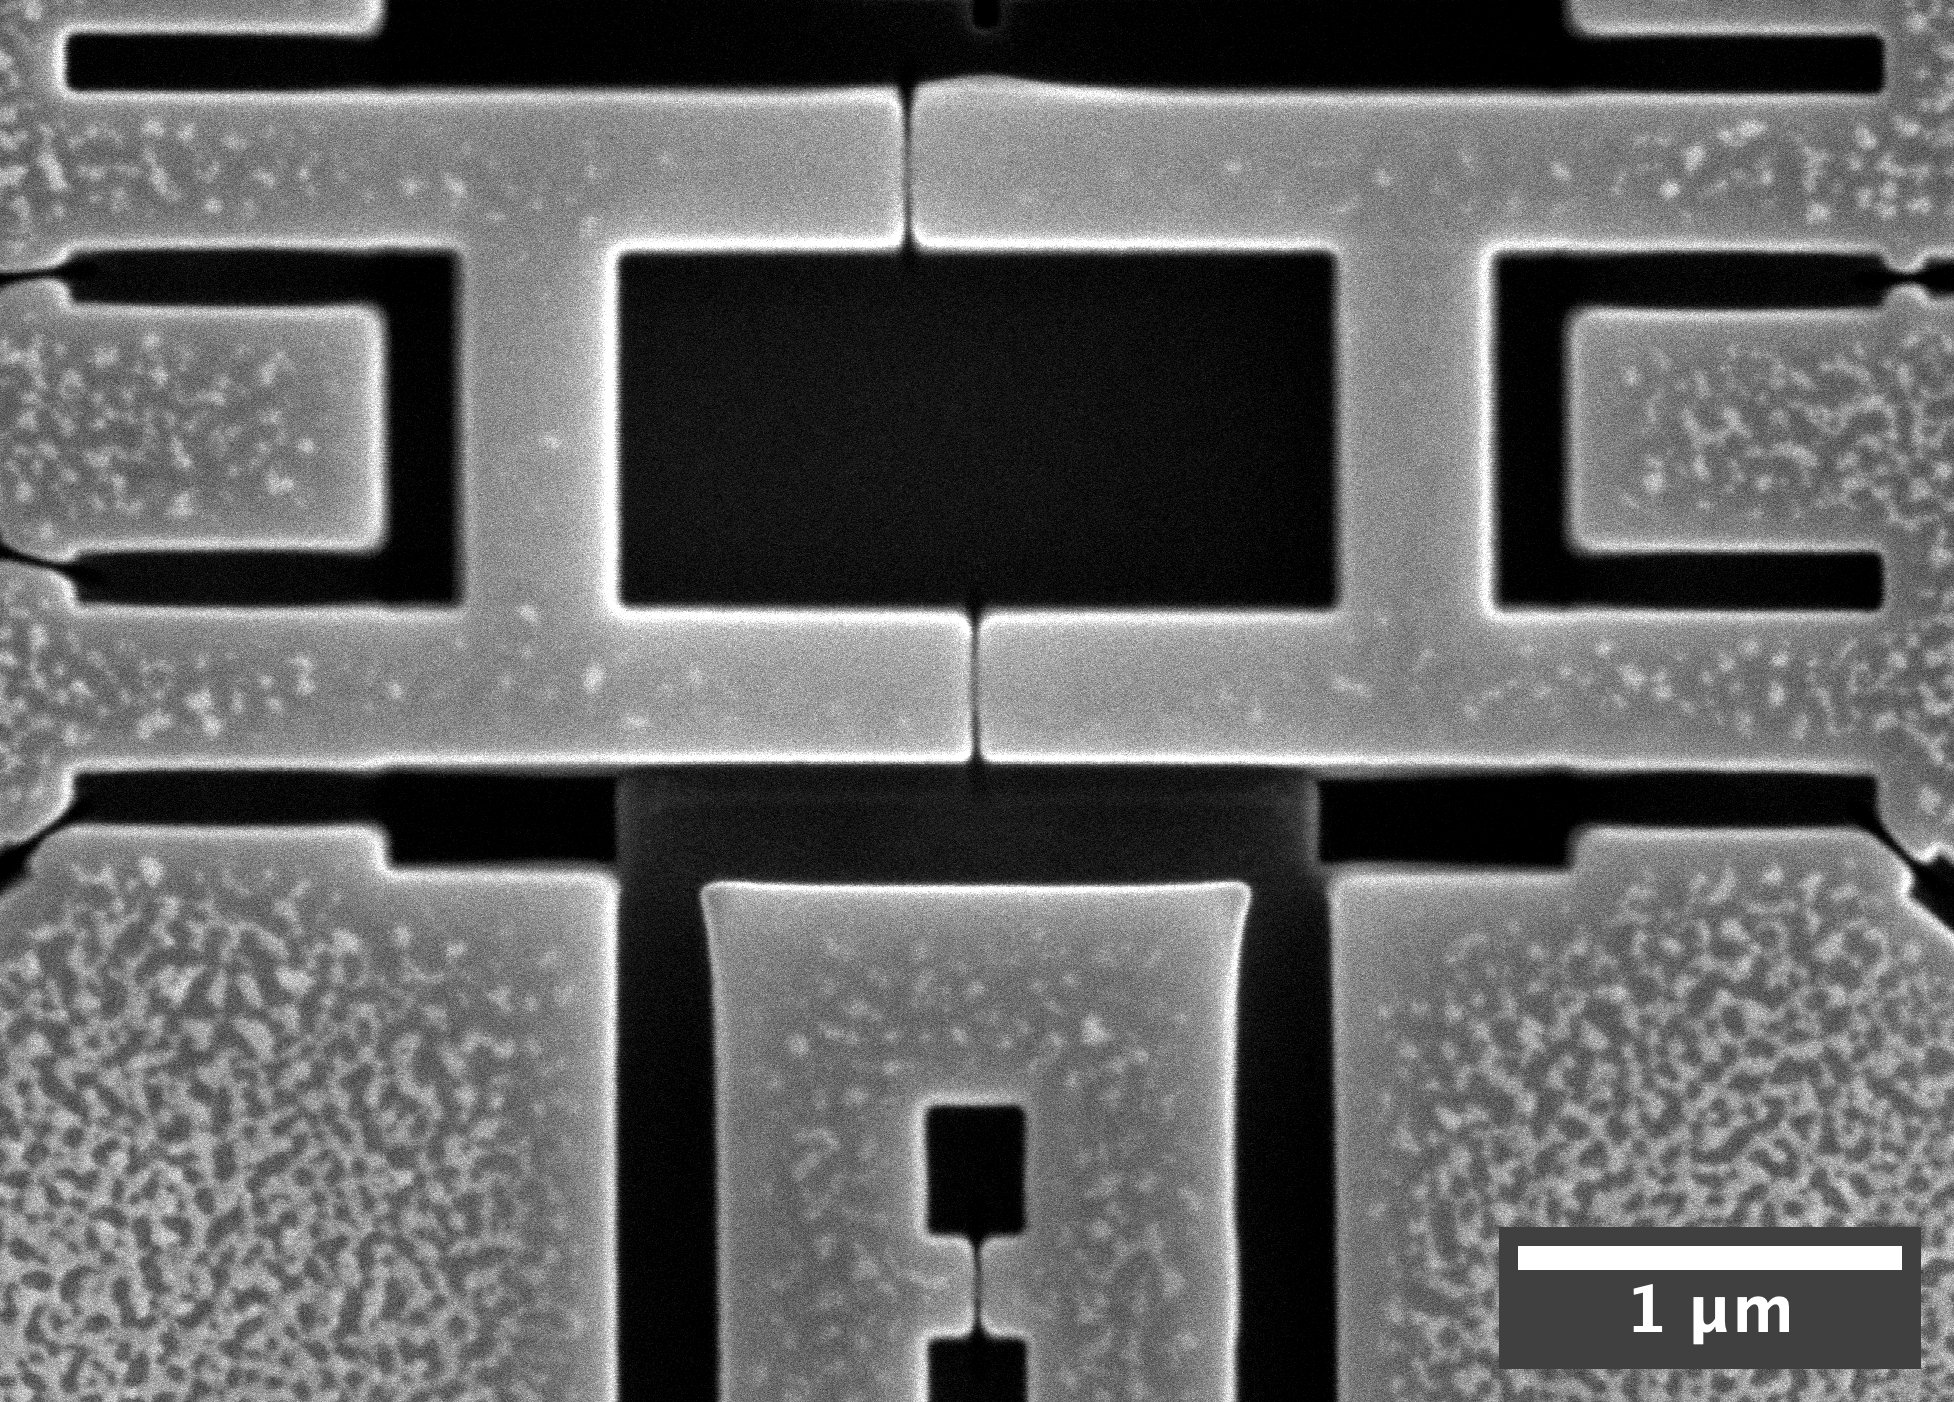
\includegraphics[width=\textwidth]{figures/samples/CP3/CP3.5A_SEM_overview.jpg}
		\subcaption{Overview of the device. The top loop shows the dc-SQUID and the bottom is the junction's loop.}
	\end{subfigure}
	\hfill
	\begin{subfigure}[t]{0.45\textwidth}
		\centering
		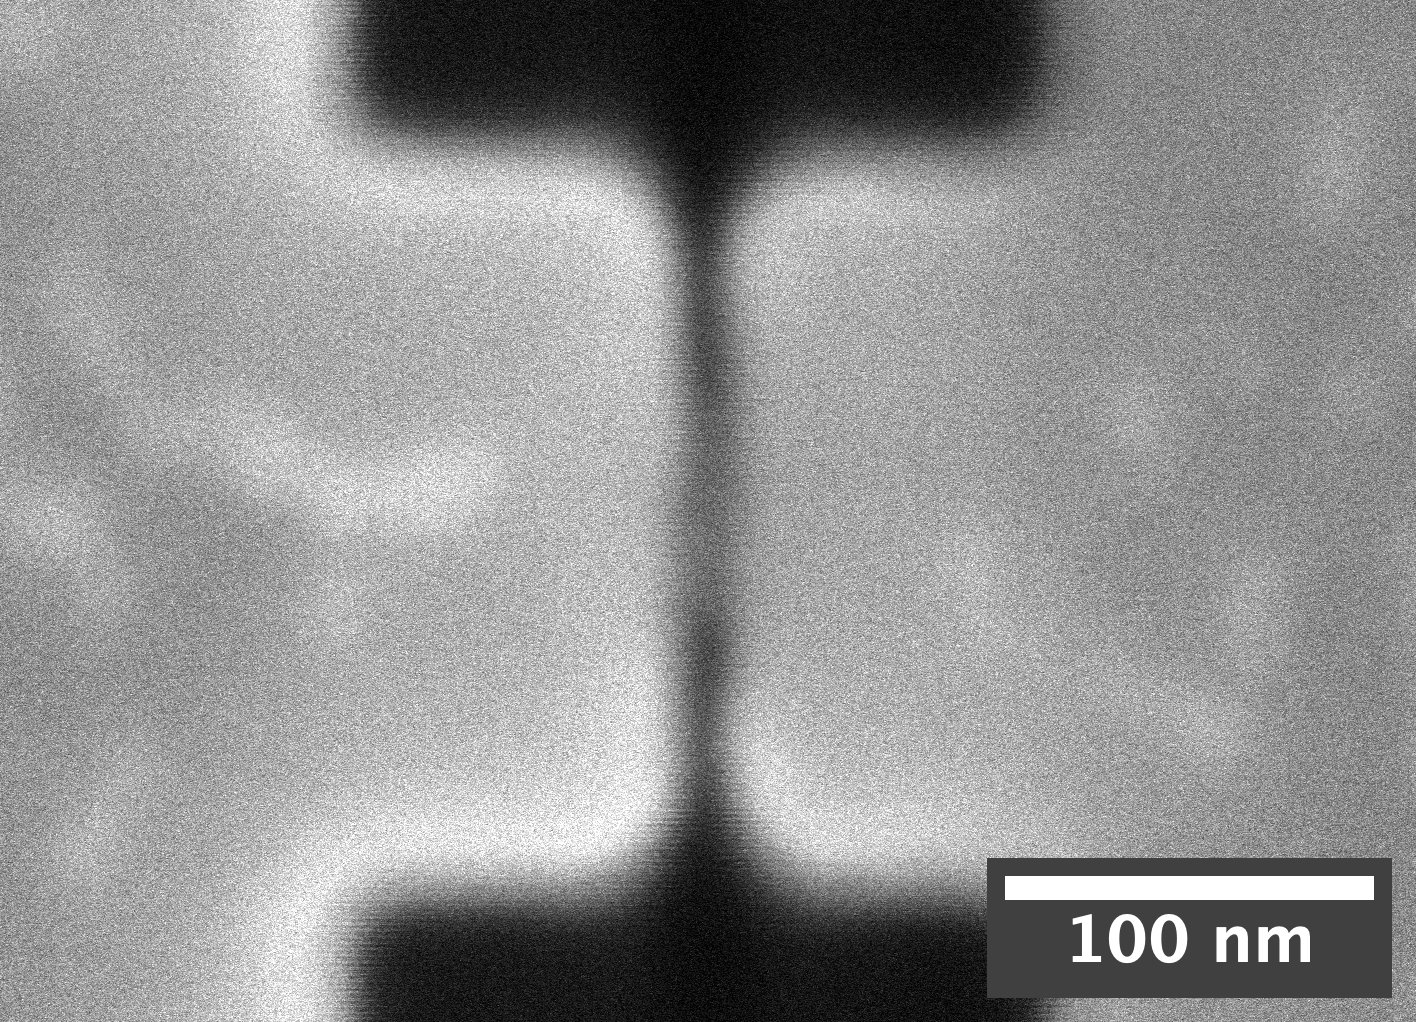
\includegraphics[width=\textwidth]{figures/samples/CP3/CP3.5A_SEM_junction.jpg}
		\subcaption{Zoomed in view of the junction, the width of the junction is \qty{12}{\nano\meter}.}
	\end{subfigure}
	
	\caption{Fine structures of sample CP3 after the FIB. Table~\ref{tab:CP3.5A-geometries} shows the exact geometries of the sample.}
	\label{fig:CP3.5A-SEM-images}
\end{figure}

\begin{table}
	\centering
	\begin{subtable}{.6\linewidth}
		\begin{tabular}[t]{@{}lrr@{}}
			\toprule
			Parameter & Value \\ \midrule
			\expandableinput tables/geometries/CP3.5A.tex
			\bottomrule
		\end{tabular}
    \end{subtable}
    \hfill
    \begin{subtable}{.3\linewidth}
    	\flushright
    	\begin{tabular}[t]{@{}lrr@{}}
    		\toprule
    		Parameter & Value \\ \midrule
    		\expandableinput tables/parameters/CP3.5A.tex
    		\bottomrule
    	\end{tabular}
    \end{subtable}
    \caption{The \textbf{left} table provides an overview of the geometries of CP3 as determined by SEM imaging and sputtering rates. The \textbf{right} table gives an overview of parameters found using a simulation based on the geometries. For the dc-SQUID two diameters are shown as it is slightly rectangular.}
    \label{tab:CP3.5A-geometries}
\end{table}